\documentclass[psamsfonts]{amsart}

%-------Packages---------
\usepackage{amssymb,amsfonts}
\usepackage[all,arc]{xy}
\usepackage{enumerate}
\usepackage[margin=1in]{geometry}
\usepackage{amsthm}
\usepackage{theorem}
\usepackage{verbatim}
\usepackage{tikz}
\usepackage{framed}
\usepackage{hyperref}
\usetikzlibrary{shapes,arrows}

\newenvironment{sol}{\vspace{0.25cm}{\large \bfseries Solution:}}{\qedsymbol}
\newenvironment{prob}[1]{\begin{framed}{\large \bfseries Problem #1:}}{\end{framed}}
\newcommand{\makenewtitle}{
    \begin{center}
    {\huge \bfseries 14.27 Economics of E-Commerce} \\
    Problem Set 2\\
    \vspace{0.25cm}
    {\bfseries John Wang} 
    \end{center}
    \vspace{0.5cm}
}

\bibliographystyle{plain}

\voffset = -10pt
\headheight = 0pt
\topmargin = -20pt
\textheight = 690pt

%--------Meta Data: Fill in your info------
\begin{document}

\makenewtitle

\begin{prob}{a-A}
Find $P^*(F')$, the optimal price the firm will charge under biased beliefs.
\end{prob}

\begin{sol}
The firm attempts to maximize expected profits, where the firm can either receive 0 if no seller is willing to buy for a price of $P$, or the firm receives $P$. Thus, the firm attempts to maximize $E[\pi | P] = P \cdot Pr[\max V_i \geq P]  = P (1 - CDF(P)) = P ( 1 - P^N)$. Taking the first order conditions, we see that $\frac{\delta \pi}{\delta P} = 1 - (N+1) P^N$. Solving for $P$ by setting the derivative equal to zero, we find that $P^*(F') = \sqrt[N]{\frac{1}{N+1}}$. 
\end{sol}

\begin{prob}{a-B}
Find $P^*(F)$, the optimal price the firm will charge under correct beliefs.
\end{prob}

\begin{sol}
We will use the same logic as before, except that this time we note that the CDF of the function is now $x/(1/2) = 2x$. Therefore, we obtain:
\begin{eqnarray}
E[ \pi | P] = P ( 1 - (2P)^N) &=& P ( 1- 2^N P^N) \\
\frac{ \delta \pi}{\delta P} &=& 1 - (N+1) 2^N P^N \\
P^*(F) &=& \frac{1}{2} \sqrt[N]{\frac{1}{N+1}}
\end{eqnarray}

Using the same process as before.
\end{sol}

\begin{prob}{a-C}
Find $E_{F'}[\pi^{posted}(F')]$, the expected profits of the posted price under biased beliefs from the point of view of the firm.
\end{prob}

\begin{sol}
Here, we can find $E_{F'}[\pi^{posted}(F')]$ by using our price with the expected probability we computed in the first part. We know that $E_{F'}[\pi^{posted}(F')] = P ( 1 - P^N)$, so we simply substitute for the $P^* = \sqrt[n]{\frac{1}{N+1}}$ that we obtained in the first part.
\begin{eqnarray}
E_{F'}[\pi^{posted}(F')] &=& P ( 1 - P^N) \\ 
&=& \sqrt[N]{\frac{1}{N+1}} \left( \frac{N}{N+1} \right)
\end{eqnarray}
\end{sol}

\begin{prob}{a-D}
Find $E_{F}[\pi^{posted}(F')]$, the expected profits of the posted price under biased beliefs but from the point of view of what will actually happen.
\end{prob}
\begin{sol}
In this case, we want to find $E_{F}[\pi^{posted}(F')] = P(1- CDF(P))$. However, we know that $CDF(P) = 2P$ by our previous arguments. This means that we have the following expression:
\begin{eqnarray}
E_{F}[\pi^{posted}(F')] &=& \sqrt[N]{\frac{1}{N+1}} \left( 1 - \left(2 \sqrt[N]{\frac{1}{N+1}} \right)^N \right) \\
&=& \sqrt[N]{\frac{1}{N+1}} \left( 1 - \frac{2^N}{N+1} \right)
\end{eqnarray}

However, this only occurs when $\sqrt[N]{\frac{1}{N+1}} < \frac{1}{2}$ because otherwise $CDF(P) = 0$. We see that $\sqrt[N]{\frac{1}{N+1}}$ is an increasing function and that $N=1$ already has $\sqrt[N]{\frac{1}{N+1}} = 1/2$. Therefore, we see that no non-negative integer values of $N$ will satisfy $\sqrt[N]{\frac{1}{N+1}} < \frac{1}{2}$. This means that no one will buy the product, and the profits will just be 0.
\end{sol}

\begin{prob}{a-E}
Find $E[\pi^{auction} (F')]$, the expected profits from the auction from the point of view of the firm. 
\end{prob}
\begin{sol}
The firm expects the buyers to have a distribution of $u[0,1]$. Since the pdf of the $k$th order statistic is $\frac{N!}{(k-1)!(N-k)!} x^k (1-x)^{N-k}$, we can find the expected profit by integrating:
\begin{eqnarray}
E[\pi^{auction} (F')] &=& \int_0^1 N(N-1) (1-x)x^{N-2} x dx \\
&=& \frac{N(N-1)}{N} - \frac{N(N-1)}{N+1} \\
&=& \frac{N-1}{N+1}
\end{eqnarray}
\end{sol}

\begin{prob}{a-F}
Find $E[\pi^{auction}(F)]$, the actual expected profits from the auction.
\end{prob}
\begin{sol}
Here, we use the same form for the probability distribution function, but we substitute $CDF(x) = 2x$ for $x$. We have the following:
\begin{eqnarray}
E[\pi^{auction}(F)] &=& \int_0^{1/2} N(N-1) (1 - (2x))(2x)^{N-2} 2x dx \\
&=& N(N-1) 2^{N-1} \left( \frac{1}{N2^N} - 2 \frac{1}{(N+1)2^{N+1}} \right) \\
&=& \frac{1}{2} (N-1) - \frac{N(N-1)}{2(N+1)} \\
&=& \frac{1}{2} \frac{(N-1)(N+1-N)}{N+1} \\
&=& \frac{1}{2} \frac{N-1}{N+1}
\end{eqnarray}
\end{sol}

\begin{prob}{a-Subpart}
Analyze the relation between C.-F. as a function of $N$, the number of bidders. It may be useful to create a table as we did in class plotting the value for different values of $N$. Identify when the firm chooses to use a posted price vs an auction: does that always work out well for the firm?
\end{prob}

\begin{sol}
We want to analyze $\sqrt[N]{\frac{1}{N+1}} \left(\frac{N}{N+1}\right) - \frac{N-1}{2(N+1)}$. The firm will choose to use a posted price when the left half of the expression is greater than the right half. This occurs when:
\begin{eqnarray}
\sqrt[N]{\frac{1}{N+1}} \left(\frac{N}{N+1}\right) &>& \frac{N-1}{2(N+1)} \\
\frac{N}{(N-1)(N+1)^{1/N}} &>& \frac{1}{2} \\
\end{eqnarray}

\begin{figure}[h!]
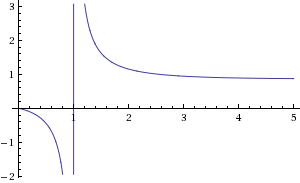
\includegraphics[width=3in]{ps2_analytical_graph.png}
\end{figure}

This occurs for all values of $N$ greater than 1. Below is a plot of the graph of $\frac{N}{(N-1)(N+1)^{1/N}}$, and it is clear that the firm will always choose the posted price for any non-negative number of buyers. Therefore, the firm will always lose out, since the auction provides larger profits for the firm. We therefore see that the firm will lose out by choosing the fixed price. 
\end{sol}

\begin{prob}{b-A}
Find $P^*(F')$, the optimal price the firm will charge under biased beliefs.
\end{prob}
\begin{sol}
This is the same question as above, so we find $P^* = \sqrt[N]{\frac{1}{N+1}}$. 
\end{sol}

\begin{prob}{b-B}
Find $P^*(F)$, the optimal price the firm will charge under correct beliefs.
\end{prob}
\begin{sol}
Now the cumulative distribution function has changed again. We now have $CDF(x)=x/2$. Therefore, we see that the expected profits are given by, $E[\pi | P] = P ( 1 - (P/2)^N)$ so that the first order conditions give:
\begin{eqnarray}
\frac{\delta \pi}{\delta P} = 0 &=& 1 - (N+1) (P/2)^N \\
P &=& 2 \sqrt[N]{\frac{1}{N+1}}
\end{eqnarray}
\end{sol}

\begin{prob}{b-C}
Find $E_{F'}[\pi^{posted}(F')]$, the expected profits of the posted price under biased beliefs from the point of view of the firm.
\end{prob}

\begin{sol}
This problem is no different than before, so we have $\sqrt[N]{\frac{1}{N+1}} \left( \frac{N}{N+1} \right)$. 
\end{sol}

\begin{prob}{b-D}
Find $E_{F}[\pi^{posted}(F')]$, the expected profits of the posted price under biased beliefs but from the point of view of what will actually happen.
\end{prob}
\begin{sol}
Again, we must change the cumulative distribution function so that $CDF(x) = x/2$. This means our expected profit is given by
\begin{eqnarray}
E_{F}[\pi^{posted}(F')] &=& P ( 1 - CDF(P)) \\
&=& \sqrt[N]{\frac{1}{N+1}} \left( 1 - \left( \frac{1}{2} \sqrt[N]{\frac{1}{N+1}} \right)^N \right) \\
&=& \sqrt[N]{\frac{1}{N+1}} \left( 1 - \frac{1}{2^{N} (N+1)} \right)
\end{eqnarray}
\end{sol}

\begin{prob}{b-E}
Find $E[\pi^{auction} (F')]$, the expected profits from the auction from the point of view of the firm. 
\end{prob}
\begin{sol}
This is no different than above, so we find $\frac{N-1}{N+1}$. 
\end{sol}

\begin{prob}{a-F}
Find $E[\pi^{auction}(F)]$, the actual expected profits from the auction.
\end{prob}
\begin{sol}
We use $CDF(x) = x/2$ and we obtain the following integral:
\begin{eqnarray}
E[\pi^{auction}(F)] &=& \int_0^2 N(N-1) (1 - x/2)(x/2)^{N-2} (x/2) dx \\
&=& \frac{N(N-1)}{2^{N-1}} \int_0^2 x^{N-1} - x^{N}/2 dx \\
&=& \frac{N(N-1)}{2^{N-1}} \left( \frac{2^N}{N} - \frac{2^{N+1}}{2(N+1)} \right) \\
&=& 2(N-1) - \frac{2N(N-1)}{N+1} \\
&=& \frac{2(N-1)}{N+1}
\end{eqnarray}
\end{sol}

\begin{prob}{3}
Blah
\end{prob}

\begin{sol}
I will be looking at the golf ball markets on eBay. I will be searching for ``Titleist ProV1 Golf Ball New 1 Dozen'' and ``Callaway Tour Golf Ball New 1 Dozen''. Both of these searches are looking for a very specific brand of golf ball, and only for a dozen of them. The searches turned up results with more than a dozen balls, in these cases I examined the price per dozen of these balls. I wrote a python script to scrape the information from eBay's website for these golf balls.

For the Titleist balls, there were 417 listings in the past 15 days, which means that there will be roughly 800 listings of this specific product each month on eBay. Note that simply searching for ProV1 golf balls yields about $5000$ results, but these are may not necessarily be new balls still in the manufacturer's packaging. I also found another auction site \url{http://www.golfbids.net/} which was auctioning off Titlesit ProV1 balls. This auction site was more geared towards buyers who were specifically in the golf ball market. It seems that the golfbids site would be able to retain more buyers, since it seems like it attempts to form a longer term relationship with buyers and allow them to continually buy golf balls from the site. However, eBay is much easier to find on Google search (finding golfbids took a couple of minutes), so simply that may make the volume of golf ball purchases on eBay larger than the volume on golfbids. However, golfbids does have a legitimate chance of overthrowing eBay as the volume leader if they are able to credibly advertise their site, and show serious golfers that they should go back to golfbids.

\begin{figure}[h!]
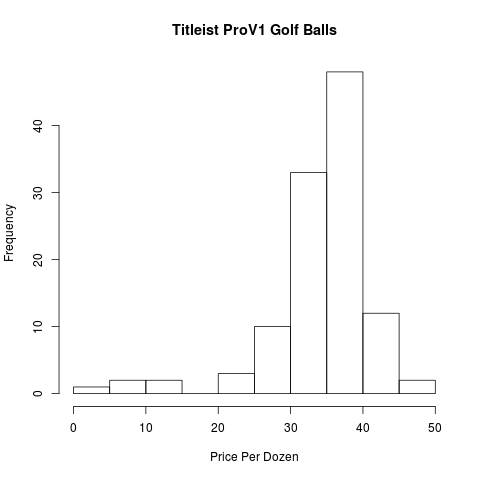
\includegraphics[width=2.5in]{unit_price_histogram.png}
\end{figure}

The standard devition of the unit price of a dozen Titleist balls was \$8.61, with an average price of \$34.74. This standard deviation is extremely large, considering that the goods are almost identical. Examining the histogram of the prices below, we can see, however, that part of the large standard deviation is due to a couple of auctions which sold the golf balls extremely cheaply. There was a cohort of people who sold these balls for prices averaging \$10 for a dozen balls. However, even removing all products sold at prices cheaper than \$20, our new standard deviation is still \$6.95 with a mean of \$35.80. This shows that the large standard deviation is fueled both by cheap sellers, and by a large disparity of prices in general.

\begin{figure}[h!]
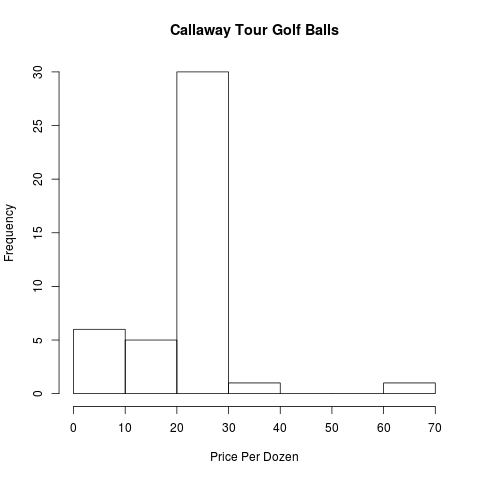
\includegraphics[width=2.5in]{unit_price_histogram_callaway.png}
\end{figure}

For the Callaway balls, the same general patterns occured. The variance was \$9.58 and the mean price was \$21.86, which means the Callaway balls had even more variance than the Titleist balls. There were 334 listings in the past 15 days, so probably about 650 listings per month. The higher variance of Callaway balls could possibly be explained by the fact that Titleist balls are more popular. In fact, Titleist balls are considered higher quality than Callaway balls, which is reflected in the average price. Possibly more people buy Callaway balls second hand, so fewer people are willing to pay a high price for them, whereas people are willing to pay a premium for the brand name of Titleist balls.

Now, if we look at the other information we have collected, we can examine whether buyer or seller reputation affects the unit price of a dozen Titleist Golf Balls. We will only examine auctions which closed and for which the product sold. We will also drop any items for which we do not have buyer or seller reputation data (many of the auctions are private). This brings us down to 65 observations in our data. We will use two covariates which represent the eBay feedback score (larger numbers mean a higher number of people have given positive feedback). These feedback scores are provided for both sellers and buyers. The results of the following regression $price\_per\_dozen_i = \alpha buyer\_score_i + \beta seller\_score_i + \epsilon$ are given below:

\begin{verbatim}
    Deviance Residuals: 
    Min       1Q   Median       3Q      Max  
    -12.910   -3.426   -0.530    1.939   44.455  
    
    Coefficients:
    Estimate Std. Error t value Pr(>|t|)    
        (Intercept)   3.561e+01  1.037e+00  34.359  < 2e-16 ***
        buyer_score  -7.229e-04  2.594e-03  -0.279    0.781    
        seller_score -6.341e-05  1.038e-05  -6.108 6.96e-08 ***
        ---
        Signif. codes:  0 ‘***’ 0.001 ‘**’ 0.01 ‘*’ 0.05 ‘.’ 0.1 ‘ ’ 1 
    
    (Dispersion parameter for gaussian family taken to be 53.76805)
    
        Null deviance: 5400.4  on 65  degrees of freedom
        Residual deviance: 3387.4  on 63  degrees of freedom
    (11 observations deleted due to missingness)
        AIC: 455.22
    
        Number of Fisher Scoring iterations: 2
\end{verbatim}

Thus, we can see that as sellers get more positive feedback, they tend to sell their products for a lower price on average. The same holds true for buyers, but the effect is not statistically significant. For sellers, this could be the case possibly because more experienced sellers are aware of the true value of the product, and believes that everyone else is overpricing. The other idea is that more experienced sellers will attempt to undercut other sellers in order to get repeat business. A final hypothesis is that experienced sellers sell in bulk, which may lower transaction costs and thus the price per unit. Performing the same regression with more covariates will help us illuminate this even more. Below, we have added controls for the percentage of letters in the title which are capital letters, and the number of annoying punctuation marks seen in the title. Annoying punctuation marks are considered anything in the set $\{!,?,*\}$.

\begin{verbatim}
    Deviance Residuals: 
    Min       1Q   Median       3Q      Max  
    -20.294   -3.526   -0.157    2.228   39.026  
    
    Coefficients:
    Estimate Std. Error t value Pr(>|t|)    
        (Intercept)                  3.549e+01  1.609e+00  22.064  < 2e-16 ***
        buyer_score                 -2.633e-04  2.598e-03  -0.101   0.9196    
        seller_score                -6.218e-05  1.038e-05  -5.991 1.21e-07 ***
        percentage_capitals         -2.065e+00  3.564e+00  -0.579   0.5644    
        number_annoying_punctuation  8.080e-01  4.716e-01   1.713   0.0917 .  
        ---
        Signif. codes:  0 ‘***’ 0.001 ‘**’ 0.01 ‘*’ 0.05 ‘.’ 0.1 ‘ ’ 1 
    
    (Dispersion parameter for gaussian family taken to be 52.81622)
    
        Null deviance: 5400.4  on 65  degrees of freedom
        Residual deviance: 3221.8  on 61  degrees of freedom
    (11 observations deleted due to missingness)
        AIC: 455.91
    
        Number of Fisher Scoring iterations: 2
\end{verbatim}

The same general results hold, and suppliers tend to sell for a lower unit price as they are more experienced. An interesting phenomenon is that more annoying punctuation tends to increase the price of an item. This may be evidence that annoying punctuation draws attention to a title. However, it may also be a remnant of self-selection bias, where people who use annoying punctuation tend to price higher in general.

Another interesting regression one can run is how the feedback score of sellers and buyers affects the bids that people make on an item. Data on the history of edge auction was collected, so that we have information on the bids that did not end up winning. If we look at the difference between the bid price and the final auction price, we can create a new distance variable $d_a$. This is a proxy for how close a bid is to actually purchasing the item. If we regress $d_a$ with the buyer and seller scores, we also find some interesting results. 

\begin{verbatim}
    Deviance Residuals: 
    Min       1Q   Median       3Q      Max  
    -29.502  -26.092  -15.493    5.065  184.716  

    Coefficients:
    Estimate Std. Error t value Pr(>|t|)    
        (Intercept)   2.952e+01  1.832e+00  16.113  < 2e-16 ***
        buyer_score  -3.390e-03  3.488e-03  -0.972  0.33146    
        seller_score -5.772e-05  1.890e-05  -3.054  0.00235 ** 
        ---
        Signif. codes:  0 ‘***’ 0.001 ‘**’ 0.01 ‘*’ 0.05 ‘.’ 0.1 ‘ ’ 1 

    (Dispersion parameter for gaussian family taken to be 1664.808)

        Null deviance: 1054361  on 625  degrees of freedom
        Residual deviance: 1037175  on 623  degrees of freedom
    (278 observations deleted due to missingness)
        AIC: 6424.8

        Number of Fisher Scoring iterations: 2
\end{verbatim}

We can see from above that a higher buyer score tends to decrease the difference between the final price and the current bid, making you closer to winning the auction. However, the effect is not statistically significant. 
\end{sol}

\begin{prob}{4}
Spend a few minutes on Google Trends exploring anything your heart contents to get warmed up. Then think of a few online companies that compete with one another and compare them using both the searches and the website features. What can you infer from the data? Can you find any interesting or surprising results?
\end{prob}
\begin{sol}
I examined the trends of Amazon.com and eBay.com. Both of these companies are similar, in that they can be categorized in the online marketing and retail industry, but they differ by the types of products they sell. For instance, eBay is more of a second hand auction site, although it is moving towards an online retail business, while Amazon has much more retail business, especially in brand name products. This distinction can provide some insight into their different Google trends.

\begin{figure}[h!]
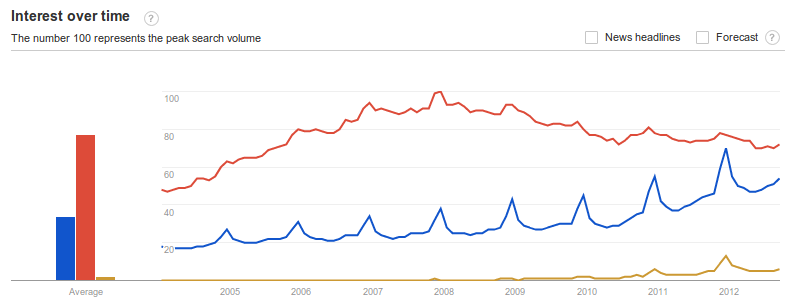
\includegraphics[width=6in]{ebay_vs_amazon.png}
\caption{eBay (Red Line) vs Amazon (Blue Line) on Google Trends}
\end{figure}

It is clear from the figure above that Amazon and eBay have completely different trends on Google searches. First, we can see that eBay seems to have reached some sort of saturation point for its growth in Google searches, whereas Amazon currently has an upward trend which is moving higher every year. This could be a reflection of the different growth phases which each company is currently in, since eBay already controls a large part of the online auction market and has few innovative products for expansion, whereas Amazon has many new technologies each year, and is pushing hard for new users. 

The other trend to notice is that Amazon is highly seasonal, whereas eBay is not. For Amazon, sales spike up without fail every December (probably due to the Christmas and Holiday season when gifts are prevalent). Ebay, however, does not perceptibly seem to be affected by seasonality. This could come from the fact that Amazon and eBay have different lines of business. In Amazon's more retail centered business, consumers usually purchase new, front-line items which were just released. Since Amazon provides a online platform for businesses to sell their latest products, consumers on Amazon are more likely to purchase gifts. However, eBay targets a set of suppliers which have an older domain of items. These are usually second hand or outdated products, which are less likely to be given as gifts. Thus, eBay sees much less of a seasonal trend, and Google searches for eBay grow much more organically.

\begin{figure}[h!]
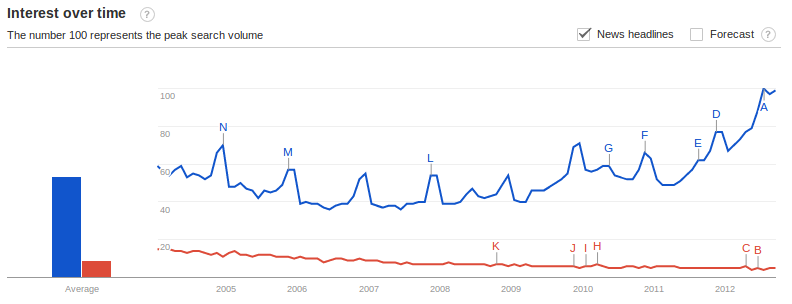
\includegraphics[width=6in]{online_shopping_vs_auction.png}
\caption{Online Auction (Red Line) vs Online Shopping (Blue Line) on Google Trends}
\end{figure}

To reinforace the hypothesis that Amazon is gaining search traction due to its business model, one can look at the Google Trends results for the terms ``Online Auction'' and ``Online Shopping''. One historically thinks of eBay as mostly an online auction site (although in recent years it has been moving to attempt to copy Amazon's model), and thinks of Amazon as a retail/shopping site. The stagnant or declining trend in people who search for ``Online Auction'' is in stark contrast to the buildup of activity in ``Online Shopping''. This last figure provides insight into why eBay and Amazon have the particular search trends that we see. These trends are correlated with the underlying business models and the type of customer that each company caters to. There has been a decline in online auctions, whereas online shopping has sped up. 
\end{sol}

\end{document}
